\documentclass{article}
\usepackage{hyperref}
\usepackage[ngerman]{babel}
\usepackage{amsmath}
\usepackage{amsfonts}
\usepackage{amsthm}
\usepackage{tcolorbox}
\usepackage[a4paper, total={7in, 9in}]{geometry}
\usepackage[font={scriptsize,it}]{caption}
\usepackage{scrextend}
\usepackage{graphicx}
\usepackage{caption}
\usepackage{subcaption}
\usepackage[utf8]{inputenc}
\usepackage[T1]{fontenc}


% floating figure for column
\newenvironment{Figure}
	{\par\medskip\noindent\minipage{\linewidth}}
	{\endminipage\par\medskip}

\theoremstyle{merke}
\newtheorem*{merke}{Merke}

\theoremstyle{definition}
\newtheorem{definition}{Definition}

\begin{document}

\begin{titlepage}
   \vspace*{\stretch{1.0}}
   \begin{center}
      \Large\textbf{Künstliche Intelligenz 1 - HS19}\\
      \large\textit{Pascal Brunner - brunnpa7}
   \end{center}
   \vspace*{\stretch{2.0}}
\end{titlepage}


\tableofcontents
\newpage



\section{Was ist AI?}
AI ist die Möglichkeit wie man Maschine beibringen kann, ähnlich wie ein Mensch zu denken und zu handeln. Dabei unterscheidet man zwischen "menschlichem" und "rationalem". Im Wesentlichen unterscheidet man \textit{denken} und \textit{handeln}. Wobei das rationale eine Mischung aus Mathematik und Engineering ist.
\textbf{mögliche Definition AI:} Ist die Diziplin für das Lösung von komplexen Problem mit dem Computer. komplexes Problem $\rightarrow$ konnte bis anhin nur der Mensch lösen

\subsection{Lernziele}
\begin{itemize}
\item tbd
\end{itemize}

\subsection{Menschliches Handeln: Der Ansatz des Turing-Test}
Der \textbf{Turing Test} wurde entwickelt, um eine zufriedenstellende betriebliche Definition von Intelligenz zu liefern. Dabei besteht ein Computer den Turing Test, wenn man die Antwort einer Person, nicht von einem Computer unterscheiden kann. Damit ein Computer diesen Test absolvieren kann, braucht er unterschiedliche Möglichkeiten:
\begin{itemize}
	\item \textbf{natural language processing} um eine erfolgreiche Kommunikation auf Englisch zu führen
	\item \textbf{knowledge representation} um neues Wissen oder neu gehörtes abzuspeichern
	\item \textbf{automated reasoning} um bereits vorhandenes Wissen für die Beantwortung von Fragen zur verwenden oder neue Erkenntnisse zu gewinnen
	\item \textbf{machine learning} um sich an neue Gegebenheiten anzupassen und Muster zu erkennen und zu erweitern
\end{itemize}
Damit ein Computer den \textbf{total Turing Test} besteht ist zusätzlich folgendes notwendig
\begin{itemize}
	\item \textbf{computer vision} um Objekte zu erkennen
	\item \textbf{robotics} um Objekte zu manipulieren und zu bewegen
\end{itemize}
$\Rightarrow$ Diese 6 Disziplinien vereinen das wichtigste zu AI.\\
Das Problem beim Turing-Test ist, dass er nicht produzierbar ist, nicht konstruktiv und sehr schwergänglich für eine klare mathematische Analyse.

\subsection{Menschliches Denken: Der kognitive Modellierungsansatz}
Wenn wir ein Programm wollen, dass wie ein Mensch denkt, so müssen wir verstehen wie der Mensch denkt. Dies kann man auf unterschiedliche Art \& Weise tätigen. 
\begin{itemize}
	\item durch Selbstbeobachtung, man probiert seine eigene Gedankengänge zu analysieren und zu verstehen
	\item durch psychologische Experimente, man beobachte einen Person "in action"
	\item durch Hirnuntersuchungen, man beobachtet das Gehirn "in action"
\end{itemize}
Sobald man eine detaillierte Anwendung des menschlichen Denkens hat, kann man entsprechend ein Programm aufsetzen. Dabei ist die interdisziplinäre cognetive Wissenschaft sehr relevant. Sie beinhaltet im Wesentlichen die Computermodelle von AI, sowie den experimentellen Techniken der Psychologie.

\subsection{Rationales Denken: Der Ansatz des Gedankengesetzes}
Es beschreibt den logischen Schluss bei einer Anzahl von Informationen. Bspw: "Socrates ist ein Mann; Alle Männer sind sterblich; Socrates ist sterblich". Dieses Gesetz des Denkens wird auch als \textbf{Logik}
 genannt. Es gibt jedoch zwei Haupthindernisse zu diesem Ansatz:
 \begin{enumerate}
 	\item Es ist nicht einfach informelles Wissen aufzubereiten, vor allem wenn das Wissen nicht 100% ist
 	\item Es ist eine grosse Differenz zwischen einem Problem prinzipiell zu lösen und ein Problem in "echt" zu lösen 
 \end{enumerate}
 
 \subsection{Rationales Handeln: Der Ansatz des rationalen Agenten}
 Ein Agent handelt einfach. Alle Computerprogramme sind Agenten, jedoch ist es nicht ein einfaches Handeln, sondern das Ziel ist es, von einem spezifischen Input den best möglichen Output zu liefern ("Das richtige tun" $\rightarrow$ Zielerreichung maximieren). Dies wird auch als \textbf{rationalen Agenten} betitelt. Beim rationalen Denken war der Schwerpunkt für AI die richtige Schlussfolgerung zu ziehen. Die richtige Schlussfolgerung zu ziehen ist in gewissen Situation Teil des rationalen Handelns, jedoch ist die richtige Schlussfolgerung nicht immer die beste Entscheidung. Es gibt Situationen wo es nicht eine offensichtliche korrekte Lösung gibt und doch muss etwas gemacht werden. Dabei gelangt man mit der richtigen Schlussfolgerung nicht zu einem Ergebnis, aus diesem Grund ist das rationale Handeln in diesen Situation zu bevorzugen. Dabei gibt es im Wesentlichen zwei Vorteile:
 \begin{enumerate}
 	\item Das rationale Handeln ist Allgemeiner gehalten als der Ansatz des rationalen Denkens, da die richtige Schlussfolgerung nur eine von vielen Möglichkeiten ist zu einer rationalen Entscheidung zu kommen. 
 	\item Das rationale Handeln ist für die wissenschaftliche Entwicklung zugänglicher als Ansätze, die auf menschlichem Verhalten oder menschlichen Gedanken basieren.
 \end{enumerate}
Ein "Ding" welches seine Umgebung wahrnimmt und kennt und entsprechend darauf reagiert $\rightarrow$ $f:P* \rightarrow A$ wobei P = Umgebung; * = gesamte Historie; A = Agent.
Der Rationale Agente ist derjenige, der das gegebene Ziel unter den gegebenen Umständen und Ressourcen bestmöglich erreicht.
\begin{itemize}
\item "schwach KI" $\rightarrow$ Ein spezifisches Problem wird versucht optimal zu lösen.
\item "Starke KI" $\rightarrow$ Es wird nicht ein spezifisches Problem gelöst, sondern man möchte eine generelle Intelligenz schaffen
\end{itemize}
\textbf{Diagramm von Slide P01 S.18}


\section{Intelligent Agents}
Im Kapitel des rationalen Handelns haben wir den rationalen Agenten kennengelernt, welchen den Ansatz verfolgt immer aufgrund seiner Gegebenheiten und seiner Umwelt "das richtige zu tun".

\subparagraph{Lernziele}
\begin{itemize}
\item Definition von rationalen Agenten und PEAS kennen
\item Ich kann erklären wieso man einen rationalen Agenten so nennt, obwohl er nicht allwissend und nicht in die Zukunft sehen kann
\item Argue how expressiveness of an agent is a mixed blessing
\end{itemize}

\subsection{Agenten und Umgebung (Environments)}
Ein \textbf{Agent} alles, was seine \textbf{Umgebung} durch \textbf{Sensoren} aufnimmt und auf das Einwirken der Umgebung mittels Aktoren reagieren kann. Im Vergleich zum Mensch sind Sensoren beispielweise:
\begin{itemize}
\item Augen
\item Ohren
\item Hände
\item uvm.
\end{itemize}
 
 \begin{merke}
 Im Allgemeinen kann die Wahl des Agenten zu einem bestimmten Zeitpunkt von der gesamten bisher beobachteten Wahrnehmungssequenz abhängen, aber nicht von etwas, das er nicht wahrgenommen hat.
 \end{merke}
 Mathematisch gesprochen wird das Verhalten des Agenten durch eine \textbf{agent function} beschrieben, welche auf eine spezifische Aktion zeigt. Aus \textit{externer Sicht} werden die Aktionen in einer Tabelle aufgelistet, welche man je nach Verhalten durchgehen kann. \textit{interne Sicht} ist ein sogenanntes \textbf{Agent Program}, bei welchem die komplette Implementation stattfindet.
 
\begin{merke}
Entscheidend ist nun, wie wir diese Tabelle ausfüllen. Was im Umkehrschluss darauf schliesst, was einen guten oder schlechten bzw. intelligenten oder dummen Agenten ausmacht.
\end{merke}

\subsection{Gutes Verhalten: Das Konzept der Rationalität}
Ein rationaler Agent macht immer das richtige, oder in andere Worte formuliert die Tabelle für die Agent function ist korrekt ausgefüllt.\\
\textit{Doch was bedeutet das Richtige tun?}
Ein möglicher Ansatz ist beim Betrachten der Konsequenz:\\
Wenn ein Agent in einer Umgebung niedergeschlagen wird, erzeugt er eine Abfolge von Aktionen entsprechend den empfangenen Wahrnehmungen. Diese Abfolge von Aktionen bewirkt, dass die Umgebung eine Abfolge von Zuständen durchläuft. Wenn die Reihenfolge korrekt ist, dann hat der Agent eine gute Leistung erbracht. Dieser Begriff der Erwünschtheit bzw. Korrektheit wird durch eine \textbf{performance measure} (Leistungskennzahl) erfasst, welche eine beliebige Folge von Umgebungszuständen auswertet.\\
\textbf{Achtung:} Man spricht von \textbf{environment states} und nicht von \textit{agent states}.\\
Beim performance measurement ist dabei wichtig, dass man klar definiert nach was gemessen werden soll. Beim einem Staubsauger beispielweise sollte man die Auswertung auf das Ergebniss legen, sprich es befindet sich keinen Dreck mehr am Boden. Und \textbf{nicht} bei den Handlungen (Dreck erkennen, aufsaugen etc.), denn so könnte die Performance gesteigert werden, in dem der Staubsauger jedes Mal wenn er alles aufgesaugt hat, wieder den Dreck ausleert und neu aufsaugt. Daher gehen wir auf das Endergebniss (= keinen Dreck mehr).\\

\begin{merke}
 In der Regel ist es besser, Leistungskennzahlen nach dem zu gestalten, was man tatsächlich tut in der Umgebung, und nicht danach, wie man denkt, wie sich der Agent verhalten sollte.
\end{merke}

\subsubsection{Rationalität}
Rationalität ist jeweils von vier Dingen abhängig:
\begin{itemize}
\item Die performance measure, welche das Erfolgskriterium festlegt
\item Die Vorkenntnisse zur Umgebung von dem Agenten
\item Die Aktionen, welche der Agent ausführt
\item Die bisherige Wahrnehmungssequenz des Agenten
\end{itemize}
Dies führt uns zu deiner \textbf{Definition für einen rationalen Agenten}
\begin{definition}
Für jede mögliche Wahrnehmungssequenz sollte ein rationaler Agent eine Aktion auswählen, von der erwartet wird, dass sie ihre Leistungskennzahl maximiert, wenn man die Beweise aus der Wahrnehmungssequenz und das eingebaute Wissen des Agenten berücksichtigt.
\end{definition}

\textbf{\textit{Beispiel: Rationaler Agent Ja / Nein?}}
\textit{Einleitende Frage: Stelle dir einen Staubsauger-Agent vor, welcher einen Raum reinigt, wenn es dreckig ist und zum nächsten Raum geht wenn er sauber ist. Ist das ein rationaler Agent?}
$\Rightarrow$ Kommt drauf an. \\
Zu erst müssen wir die performance measure, Umgebung, Sensoren und Aktoren definieren.
\begin{itemize}
\item Die performance measure erhält einen Punkt für jeden gereinigtes Raum, welcher innerhalb von 1000 Zeitschritten erfolgen konnte
\item Die geografische Lage der Umgebung ist a priori bekannt, jedoch die Dreckverteilung sowie der Ausgangspunkt des Agenten nicht. Saubere Räume bleiben sauber und reinigen den aktuell Raum weiter. Links und Rechts bewegen den Staubsauger nach links und rechts, ausser wenn diese Bewegung das Verlassen der Umgebung veranlassen würde, dann würde der Agent dort bleiben wo er sich aktuell befindet
\item Die einzigen Aktionen sind links, rechts und saugen
\item Der Agent erkennt seine Position richtig und ob diese Schmutz enthält oder nicht
\end{itemize}
$\Rightarrow$ Unter diesen Umständen handelt es sich um einen rationalen Agenten

\subsubsection{Allwissenheit, Lernen und Autonomie}
Es gilt die beiden Begrifflichkeiten \textit{Rationalität} und \textit{Allwissenheit} klar zu unterscheiden.
\begin{itemize}
\item \textbf{Allwissendheit} - Der Agent kennt den aktuellen Outcome seiner Aktion und kann sofort darauf reagieren. $\rightarrow$ dies ist in der Realität jedoch unrealistisch
\item \textbf{Rationaltität} - Bei der Rationalität geht es darum, seine erwartende Performance zu maximieren, dies während der aktuellen Performance. Diese lässt sich jedoch nicht perfektionieren. Die Rationalität setzt nicht Allwissenheit vorraus.
\end{itemize}
Ein wichtiges Ereignis bei der Rationalität ist das \textbf{information gathering}. Für unseren Agent ist jedoch nicht nur das Sammeln von Informationen elementar, sondern auch das \textbf{Lernen}. Er sollte so viel als mögliche von der erhaltenen Informationen lernen. Dabei können wir dem Agenten ein Basis-Wissen an Informationen liefern, welcher er selbstständig mit den gewonnen Informationen ausbauen kann. \\
In dem Masse, in dem sich ein Agent auf das Vorwissen seines Designers und nicht auf seine eigenen Vorstellungen verlässt, sagen wir, dass es dem Agenten an \textbf{Autonomie} mangelt. Ein rationaler Agent sollte jedoch in der Lage sein autonom zu sein - er sollte lernen er von dem bereits bestehenden Wissen kompensieren kann bzw. falsches Wissen zu korrgieren und dadurch sein Wissen weiteraufbauen. Nach ausreichender Erfahrung in seiner Umgebung kann das Verhalten eines rationalen Agenten effektiv unabhängig von seinem Vorwissen werden.\\

Nun steht die Definition der Rationalität und wird haben die Basis um einen rationalen Agent zu bauen. Zuerst müssen wir uns jedoch noch mit dem \textbf{task environment} befassen, welches das \textit{essenzielle Problem} für den rationalen Agenten ist, welches er zu lösen hat.

\subsubsection{Task environment spezifizieren}
Die spezifizierten performance measure, the environment und der Agent's actuators und Sensoren, werden alle unter \textbf{task environment} zusammengefasst. Dies wird auch \textbf{PEAS} (\textbf{P}erformance, \textbf{E}nvironment,\textbf{A}ctuators,\textbf{S}ensors) genannt. Während dem Designen eines Agenten, muss zu aller erst immer das task environment so gut als möglich spezifiziert werden. Gerade auch als Ausblick für den Aufbau einer KI, sind die PEAS-Kriterien sehr wichtig. Analog dem Aufbau eine Business Cases, bevor man mit einem Unternehmen beginnnt.

\textbf{\textit{Beispiel: automatischer Taxi Fahrer}}
Die einzelnen Punkte werden nachfolgend erläutert
\begin{Figure}
\centering
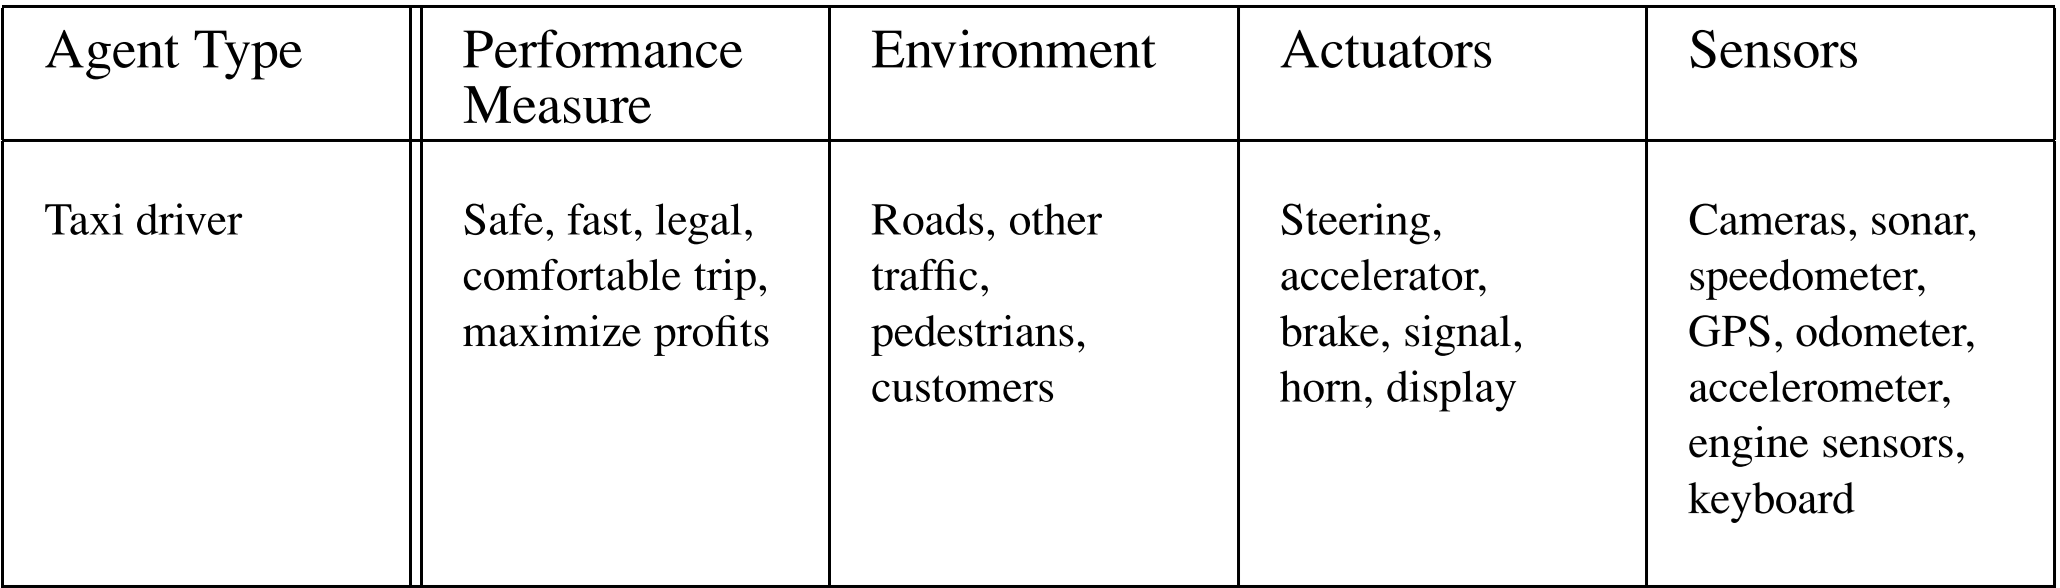
\includegraphics[width=400px]{img/taskEnvironmentTaxi.png}
	\captionof{figure}{PEAS Beschreibung für task environment bei einem automatisierten Taxi-Fahrer}
	\label{fig:PEAS Beschreibung}
\end{Figure}

\begin{enumerate}
\item \textbf{performance measure} - \textit{was streben wir an?}
\begin{itemize}
\item Korrekte Destination
\item Minimaler Gebrauch von Benzin, so wie möglich geringe Abnutzung
\item Minimale Kosten bzw. Zeit pro Reise
\item Möglichst keine Übertretungen der Strassengesetze 
\item Maximale Sicherheit und Komfort
\item Maximaler Profit
\end{itemize}
$\Rightarrow$ Es gibt einige Zielkonflikte, wo durch Kompromisse eingegangen werden müssen
\item \textbf{Environment} - \textit{Wie sieht die Umgebung des Taxi's aus?}
\begin{itemize}
\item Unterschiedliche Strassenarten (von Kinderzonen bis zur mehrspurigen Autobahn)
\item Zusätzliche Verkehrsteilnehmer (Passanten, andere Fahrzeuge, priorisierte Fahrzeuge Polizei etc.)
\item Veränderungen der Gegebenheiten wie bspw. Wetter
\item Multi-Nationaler Einsatzmöglichkeiten (bspw. Linksfahren in England)
\end{itemize}
$\Rightarrow$ Je mehr wir die Umgebung eingrenzen, desto einfacher werden die Design-Probleme
\item \textbf{Actuators} - \textit{Welche Möglichkeiten muss es geben?}
\begin{itemize}
\item Kontrolle über den Motor, das Steuerrad, sowie den Bremsen
\item Interaktionsmöglichkeiten (Bspw. Sprachgenerator zum mit den Passanten zu kommunizieren oder Displays für andere Verkehrsteilnehmer)
\end{itemize}
\item \textbf{Sensors} - \textit{Was muss das Taxi von seiner Umgebung aufnehmen können?}
\begin{itemize}
\item Mehrere kontrollierbare Kameras für die Aufnahme der Strasseneinflüsse
\item Distanzmessungen zu anderen Objekten
\item Erkennung der aktuellen Geschwindigkeitsbegrenzung inkl. Anpassung seiner Geschwindigkeit
\item Beschleunigungssensor, welcher auch bei Kurven o.ä. eingreift
\item Kontrolle über den Zustand des Autos (Benzin, Öl, Reifen, Bremsen, uvm.)
\item GPS
\item Mikrofon und Tastatur für die Eingabe zum gewünschten Ziel
\end{itemize}
\end{enumerate}
$\Rightarrow$ Es werden diverse Agenten gebraucht um dies umsetzen zu können. Dabei kommen oftmals die Diskussionen auf, ob es sich um einen rationalen oder einen intelligenten Agenten handelt. Tatsächlich geht es nicht um die Unterscheidung zwischen "realen" und "künstlichen" Umgebungen, sondern um die Komplexität der Beziehung zwischen dem Verhalten des Agenten, der von der Umgebung erzeugten Wahrnehmungssequenz und dem Leistungsmass.

\subsubsection{Eigenschaften der task environments}
Die Anwendungsbereich in welchen KI eine Aufgaben übernehmen können sind enorm breit gefächert und vielfältig. Nachfolgend sind einige Agenten-Typen aufgelistet inklusive deren Beschreibung für die Eingliederung im PEAS.

\begin{Figure}
\centering
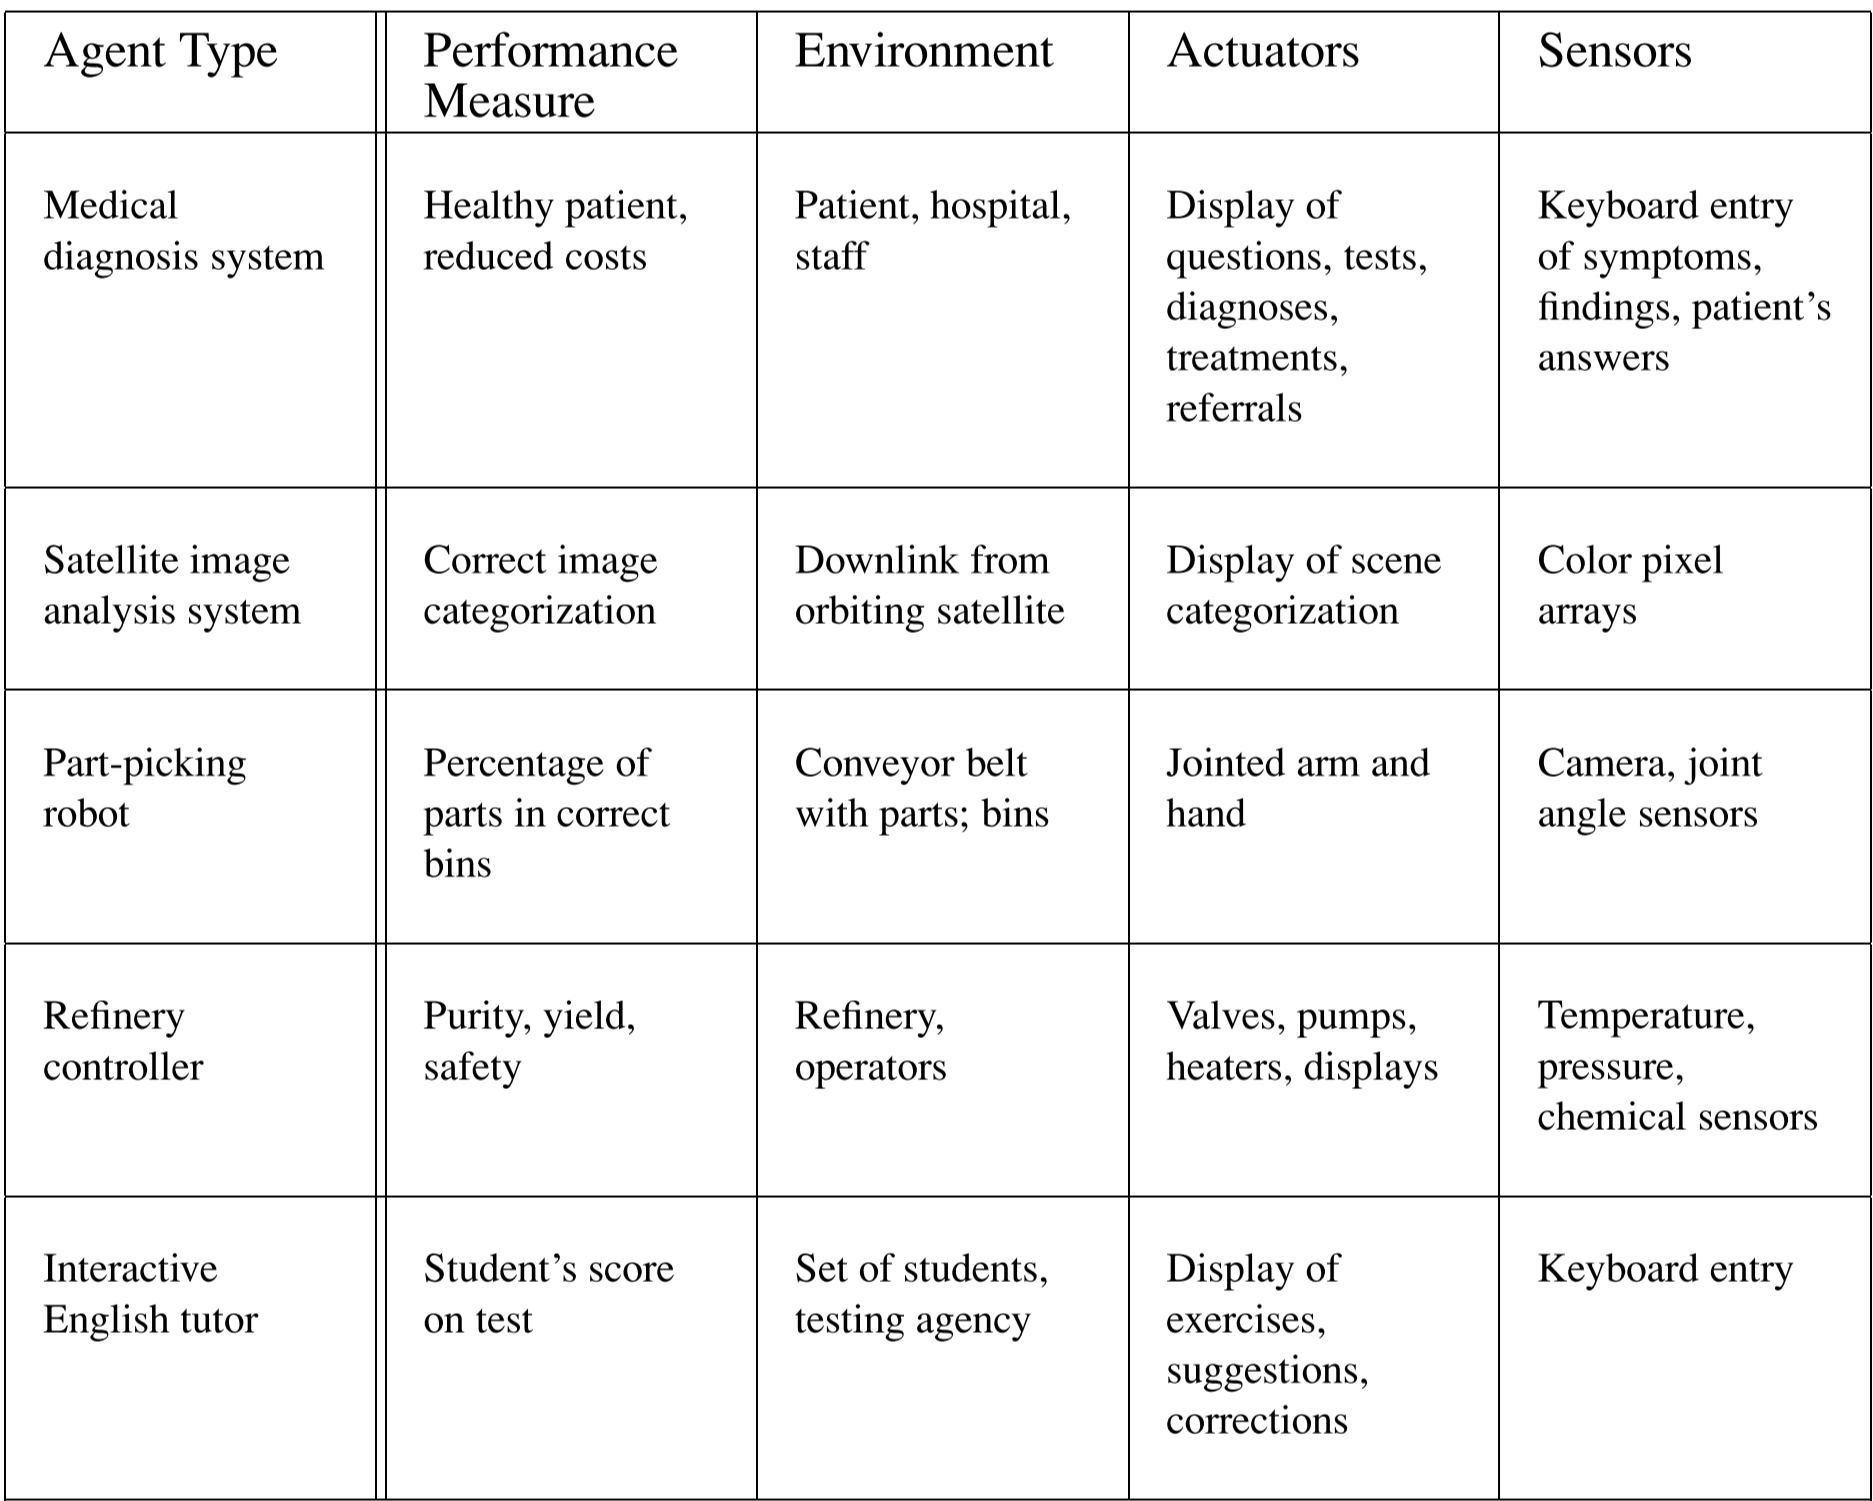
\includegraphics[width=300px]{img/AgentTypes.png}
	\captionof{figure}{Beispiele von AgentenTypen und deren PEAS Beschreibung}
	\label{fig:Beispiele von AgentenTypen und deren PEAS Beschreibung}
\end{Figure}

\textbf{Fully observable vs. partially observable}
\begin{itemize}
\item Wenn ein Sensor zu jedem Zeitpunkt sämtliche \textit{relevanten} Informationen zurück liefert um die Auswahl der betreffenden Aktion auszuwählen, sprechen wir von einem \textbf{fully observable} Umgebung.\\
$\Rightarrow$ fully observable Umgebungen sind sehr praktisch, da keine interne Zustände gespeichert werden müssen. Bspw. ist Schach fully observerable, jedoch Poker nicht. Da man beim Poker verdeckte Karten hat.
\item Sobald eine Informationen fehlen oder zu ungenau sind, so sprechen wir von einer \textbf{partially observable} Umgebung
\item Wenn der Agent keine Sensoren hat, sprechen wir von einer \textbf{unobservable} Umgebung.
\end{itemize}

\textbf{Single Agents vs. Multiagent}\\
Diese Unterscheidung fällt einem leicht zu treffen. Wenn nur ein Agent gebraucht wird um das Problem zu lösen, so wird von einem single Agent gesprochen. Bei den Mutliagents differenzieren wird noch zwischen verschiedenen Betrachtungen. 
\begin{itemize}
\item competitive (konkurrierend)
\item cooperative (kooperativ)
\end{itemize}
$\Rightarrow$ Beispielsweise im Eishockey spielt ein Team (Teamintern kooperativ) gegen ein anderes Team (konkurrierend).\\

\textbf{Deterministisch vs. Stochastik vs. nondeterministic}
Wenn der nächste Zustand der Umgebung vollständig durch den aktuellen Zustand und die vom Agenten ausgeführte Aktion bestimmt wird, dann sagen wir, dass die Umgebung \textbf{deterministisch} ist, sonst nennen wir es \textbf{stochastisch}. Das Taxi-Beispiel ist klar stochastisch getrieben, da man nie eindeutig voraussagen kann wie das Verhalten des Verkehrs ist.\\
\textit{nondeterministic}\\
Dinge die bspw. sehr schwer zum Berechnen, sind da die Berechnung sehr komplex ist, wird nicht-deterministisch (man kann keine genaue Wahrscheinlichkeit angeben)\\
Wir sagen, dass die Umgebung \textbf{unklar / unsicher} ist, wenn die Umgebung nicht fully observale oder nicht deterministisch ist.\\

\textbf{episodisch vs. sequentiell}\\
Bei einer \textbf{episodischen} Ausführung eines Tasks ist jeder Task in sich geschlossen (atomic).  Dementsprechend ist die nächste Aufgabe faktisch unabhängig der vorherigen. Bei der \textbf{sequentiellen} Ausführung kann eine Entscheidung im Task x, alle nachfolgenden Entscheidungen und Ausführunen beinflussen.\\

\textbf{static vs. dynamic}\\
Wenn die Umgebung sich ändern kann, während ein Agent 'nachdenklich' ist, so sprechen wir von einer \textbf{dynamischen} Umgebung. Sonst handelt es sich um eine \textbf{statische} Umgebung.\\

\textbf{diskret vs. kontinuierlich}\\
Die Unterscheidung zwischen diskret und kontinuierlich ist abhängig des \textit{state} von der Umgebung, der \textit{Zeit} in welcher es handelt, sowie der \textit{Wahrnehmungen} und \textit{Aktionen} des Agenten.\\

\textbf{bekannt vs. unbekannt}\\
In einer \textbf{bekannten} Umgebung, sind die Ergebnisse (oder die Ergebnisse für alle Möglichkeiten in einer stochastischen Umgebung) für alle Aktionen gegeben. Wobei in einer \textbf{unbekannten} Umgebung der Agent seine Umgebung zuerst noch kennenlernen muss. Es ist jedoch auch möglich, dass es sich um eine \textit{bekannte, partially observable} Umgebung handelt, bspw. Solitaire. $\rightarrow$ Ich kenne die Regeln, bin jedoch nicht im Stande zu sehen, was als nächste Karte kommt. Des Weiteren gibt es auch \textit{unbekannte, fully observable} Umgebungen, bspw. Video-Spiele. $\rightarrow$ Ich sehe den kompletten Bildschirm, aber ich weiss trotzdem nicht welche Auswirkungen die einzelne Knöpfe haben, bis ich diese ausprobiert habe.

\begin{Figure}
\centering
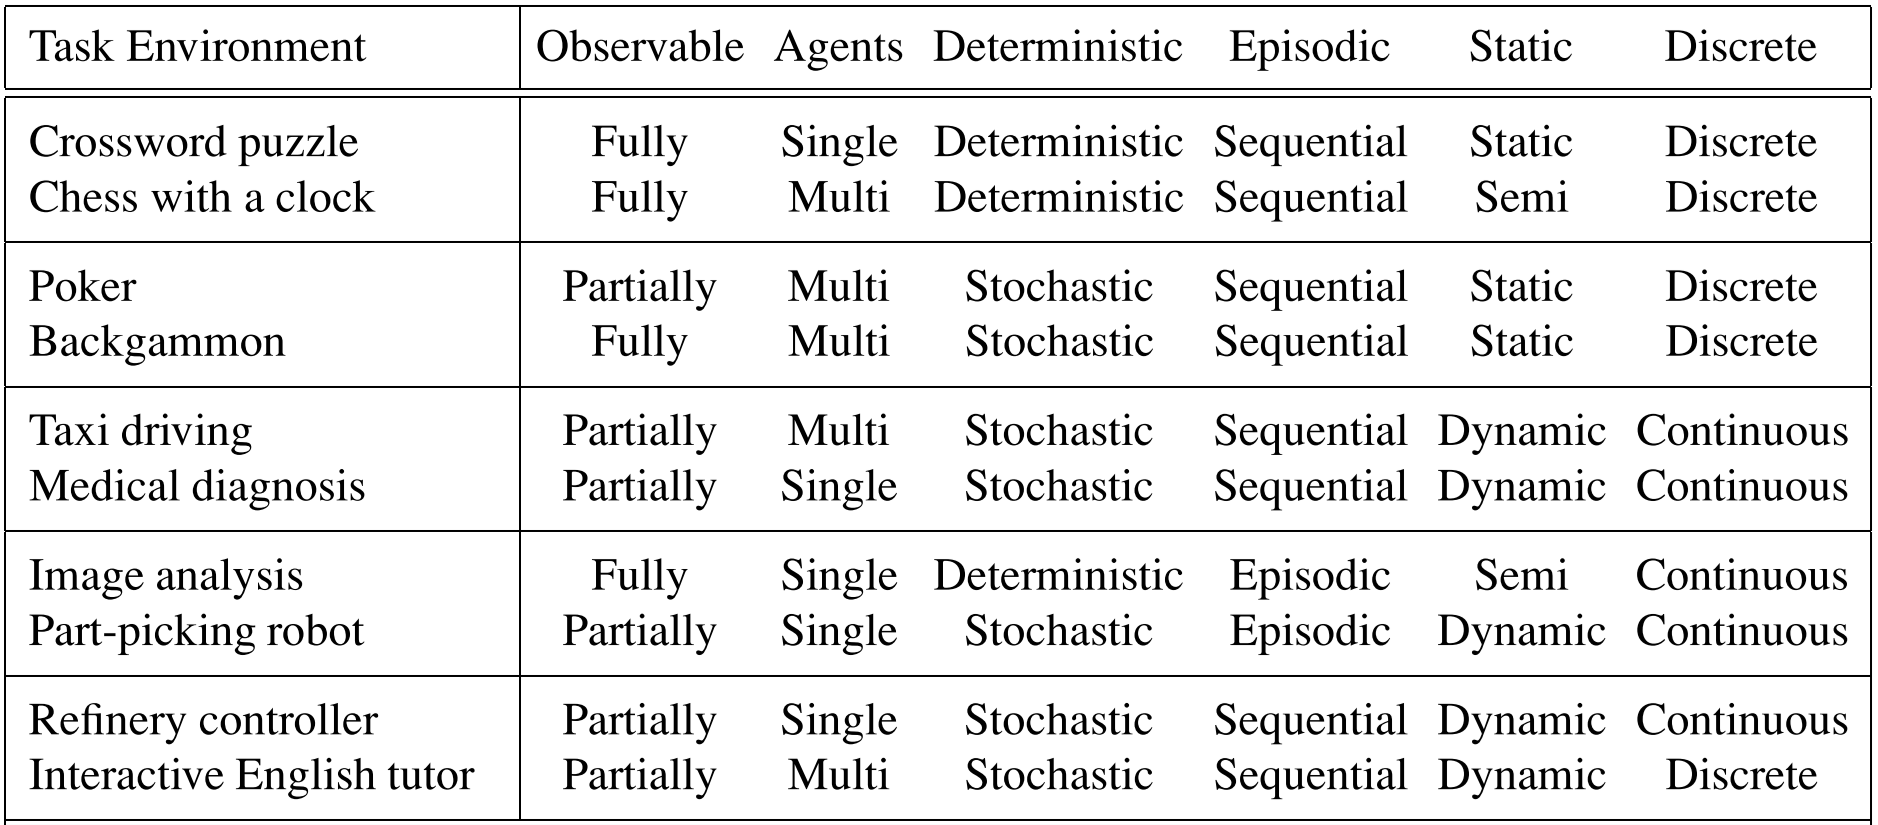
\includegraphics[width=300px]{img/TaskEnvironmentsCharacteristics.png}
	\captionof{figure}{Beispiele von Task Environsments mit deren charakteristik}
	\label{fig:Beispiele von Task Environsments mit deren charakteristik}
\end{Figure}

\subsection{Die Struktur der Agenten}
Der Job von KI ist es, ein \textbf{agent program} zu designen, welches die agent function implementiert (Mapping von Wahrnehmung zu Aktion). Wir nehmen an, dass dieses Programm auf einem Computer-Gerät mit physikalischen Sensoren und Actuators läuft. Dies nennen wir \textbf{Architektur}:\\
$ agent = architecture + program$
Natürlich müssen wir unser Programm so wählen, welches auf die entsprechende Architektur angepasst ist. Wenn wir eine Aktion ausführen \textit{laufen}, so wäre es besser, wenn die Architektur Beine hat.

\subsubsection{Agent programs}
Agent Programs, welche wir hier designen haben alle dasselbe Grundgerüst: Sie nehmen die aktuelle Wahrnehmung als Input der Sensoren auf und wiedergeben diese mittels einer Aktion an die Aktoren.
\begin{Figure}
\centering
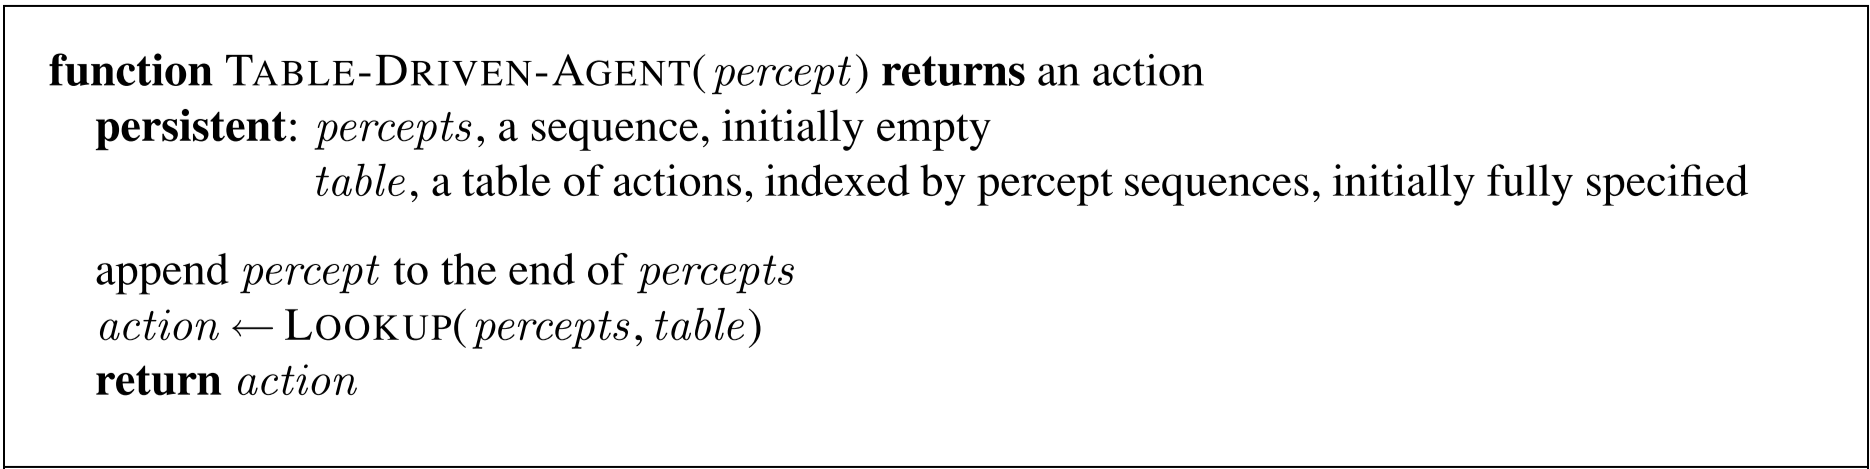
\includegraphics[width=300px]{img/TableDrivenAgent.png}
	\captionof{figure}{Beispieltabelle für Table Driven Agent}
	\label{fig:Beispieltabelle für Table Driven Agent}
\end{Figure}
Wenn wir den Einsatz von einem Table-Driven Ansatz genauer anschauen, merken wir, dass dieser in der Praxis nicht verwertbar ist. 
Definieren wir $P$ als mögliche Wahrnehmungen und $T$ als Lifetime des Agenten (so viele Wahrnehmungen wird der Agent erhalten). Die LookUp Table wird mit folgender Grösse befüllt: $\sum\limits_{t=1}^{T} |P|^T$. Wenn wir nun ausgehen, dass in bei einem Taxi-Fahrer eine Kamera pro Sekunde 27MegaBytes an informationen liefert, ergibt das eine Tabelle von $10^{250'000'000}$ Einträge. $\rightarrow$ keine Tabelle auf der Welt kann diese Menge an Datenspeichern.\\

Und doch, der Tabellen-Ansatz macht das was wir wollen $\rightarrow$ es implementiert die gewünschte agent function. Der Hauptherausforderung bei KI ist, dass wir einen guten Weg finden wie wir das Programm schreiben, welches alle Möglichkeiten abdeckt und nach rationalem Verhalten funktioniert.

\subsubsection{simple reflex agents}
Die einfachste Art eines Agenten ist der simple reflex agent. Dieser Agent wählt die Aktion auf Basis der \textit{aktuellen} Wahrnehmung aus, und ignoriert dabei die komplette Historie. Wenn wir wieder Bezug nehmen auf den Staubsauger, war dieser ein simple reflex agent. Denn er entschied auf Basis der aktuellen Situation und ob diese Dreck enthalten hat oder nicht. Dabei ist die Reduzierung auf das Vernachlässigen der Historie mit der grössten Auswirkung betroffen. Denn die Anzahl von Möglichkeiten $4^T$ wurde auf 4 reduziert. \\
$\Rightarrow$ Reflex, es passiert etwas ohne darüber nachzudenken (Beim Menschen bspw. das Blinzeln, Husten etc.)\\
Simple reflex agent kommen jedoch auch in komplexeren Umgebungen vor. Wenn wir uns wieder an das Taxi-Beispiel erinnern, so wäre ein mögliches Szenario, dass wenn das Auto vor mir bremst und sein Bremslicht angeht, dass ich dies erkennen muss und ebenfalls bremsen muss.\\
\textit{\textbf{if} car-in-front-is-breaking \textbf{then}   initiate-breaking}\\
\begin{Figure}
\centering
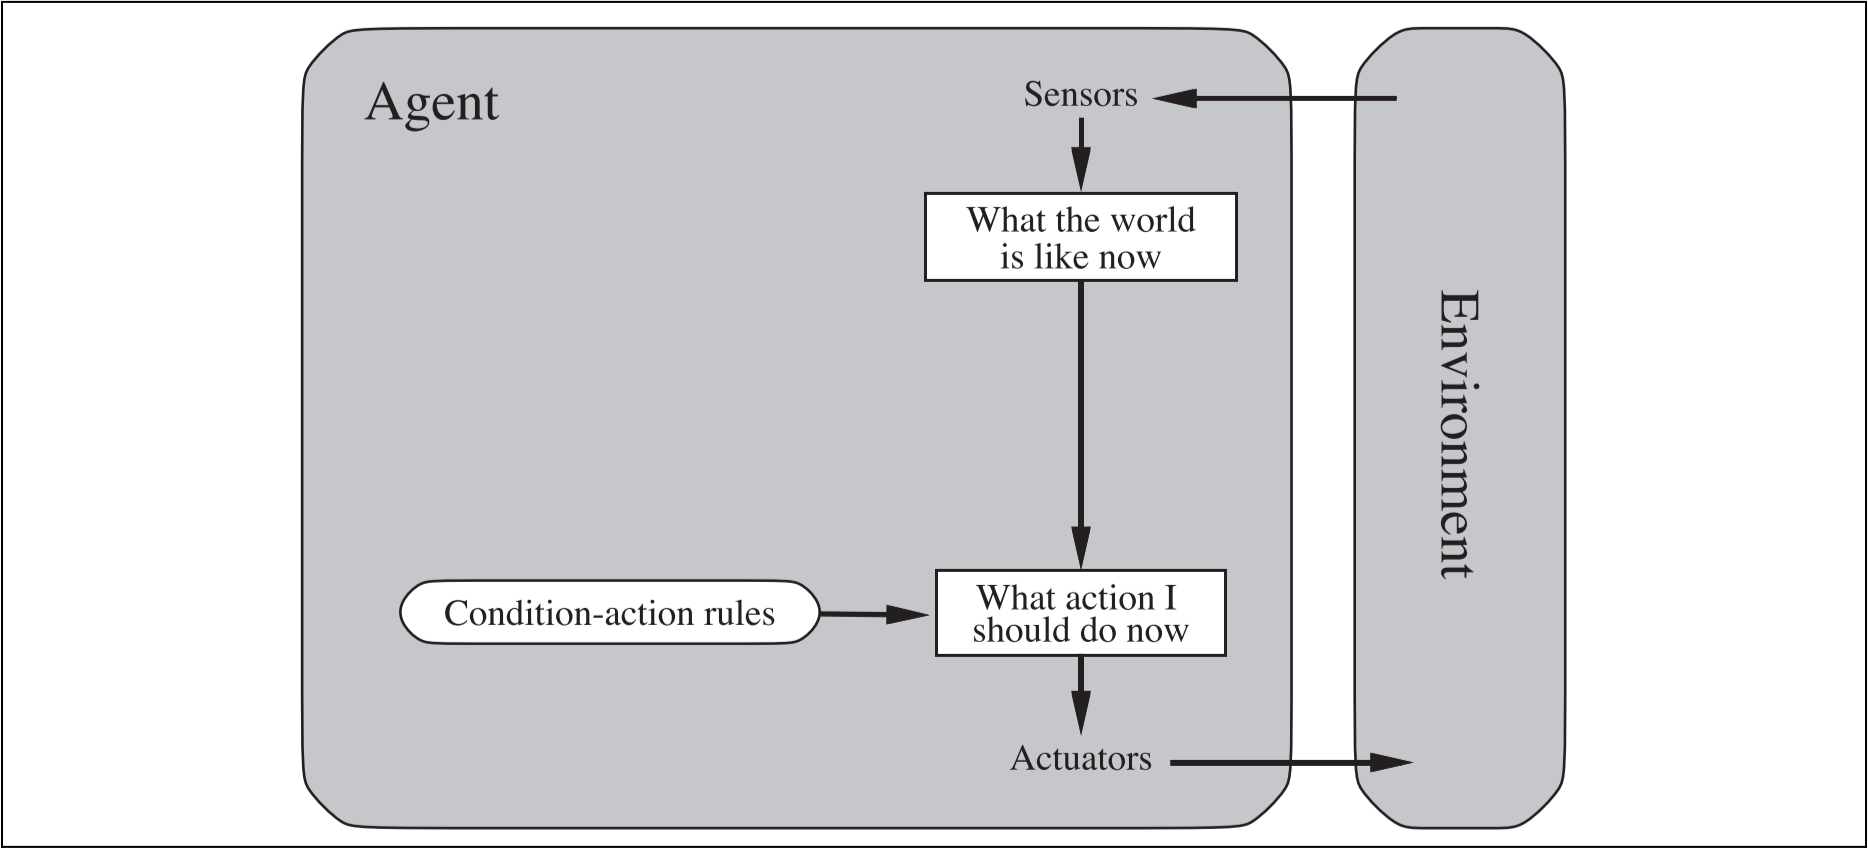
\includegraphics[width=400px]{img/SchemaSimpleReflexAgent.png}
	\captionof{figure}{Schema eines Simple Reflex Agent}
	\label{fig:Schema eines Simple Reflex Agent}
\end{Figure}
\begin{Figure}
\centering
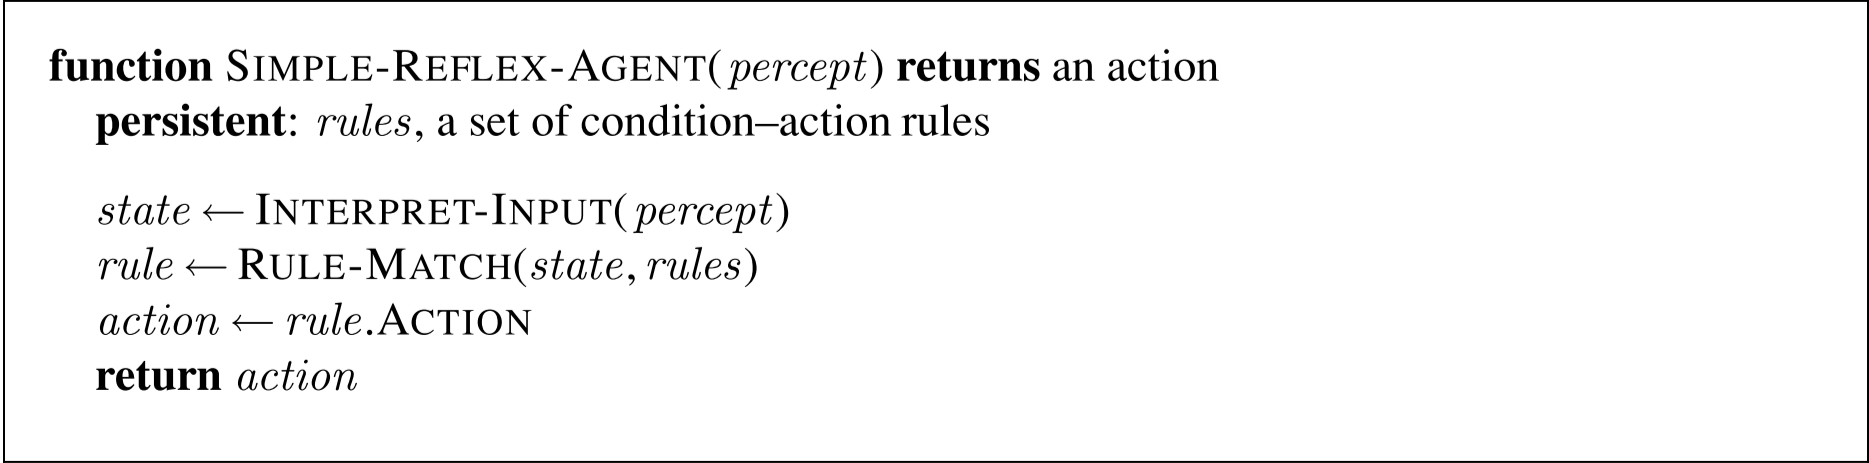
\includegraphics[width=300px]{img/FunctionSimpleReflexAgent.png}
	\captionof{figure}{Function eines Simple Reflex Agent}
	\label{fig:Function eines Simple Reflex Agent}
\end{Figure}

\section{Problemlösung mittels Suche}
Die Suche ist ein klassicher KI-Ansatz, welcher schon seit einiger Zeit im Einsatz ist und trotzdem hat es seine starke Berechtigung.\\

\subsection{Lernziel}
\begin{itemize}
\item Kennen der klassischen Such-Algorithmen und wie sie sich hier in der Komplexität (Speicher und Zeit) unterscheiden
\item Verstehen wie ein intelligentes Verhalten funktioniert
\item kennen wie man eine Suche mittels einer Heuristik verbessern kann.
\item Modellierung auf ein Real-World Beispiel anwenden kann
\end{itemize}

\subsection{Suche als Problemlösung}
Beispielsweise das GPS-Problem mit einer Anfangsstadt (\textbf{Initial State}) und einer finalen Destination (\textbf{formulate goal}). Das Problem wird mittels dem Formulieren des Problems, mittels verschiedenen \textbf{States} (Städte) und \textbf{actions} (Fahrt zwischen den Städten).\\

Dabei beginnt man zuerst mit der \textbf{Formulierung des Problems}.
\begin{enumerate}
\item initial state $\rightarrow$ man befindet sich in Arad
\item successor function $\rightarrow$ gibt uns die verschiedenen Möglichkeiten an
\item goal test $\rightarrow$ explizit (Zielstadt ist Bukarest) oder implizit (nicht mehr dreckig)
\item path cost $\rightarrow$ aufsummierte Kosten der Distanz oder die Anzahl der Aktionen etc.
\end{enumerate}
\begin{Figure}
\centering
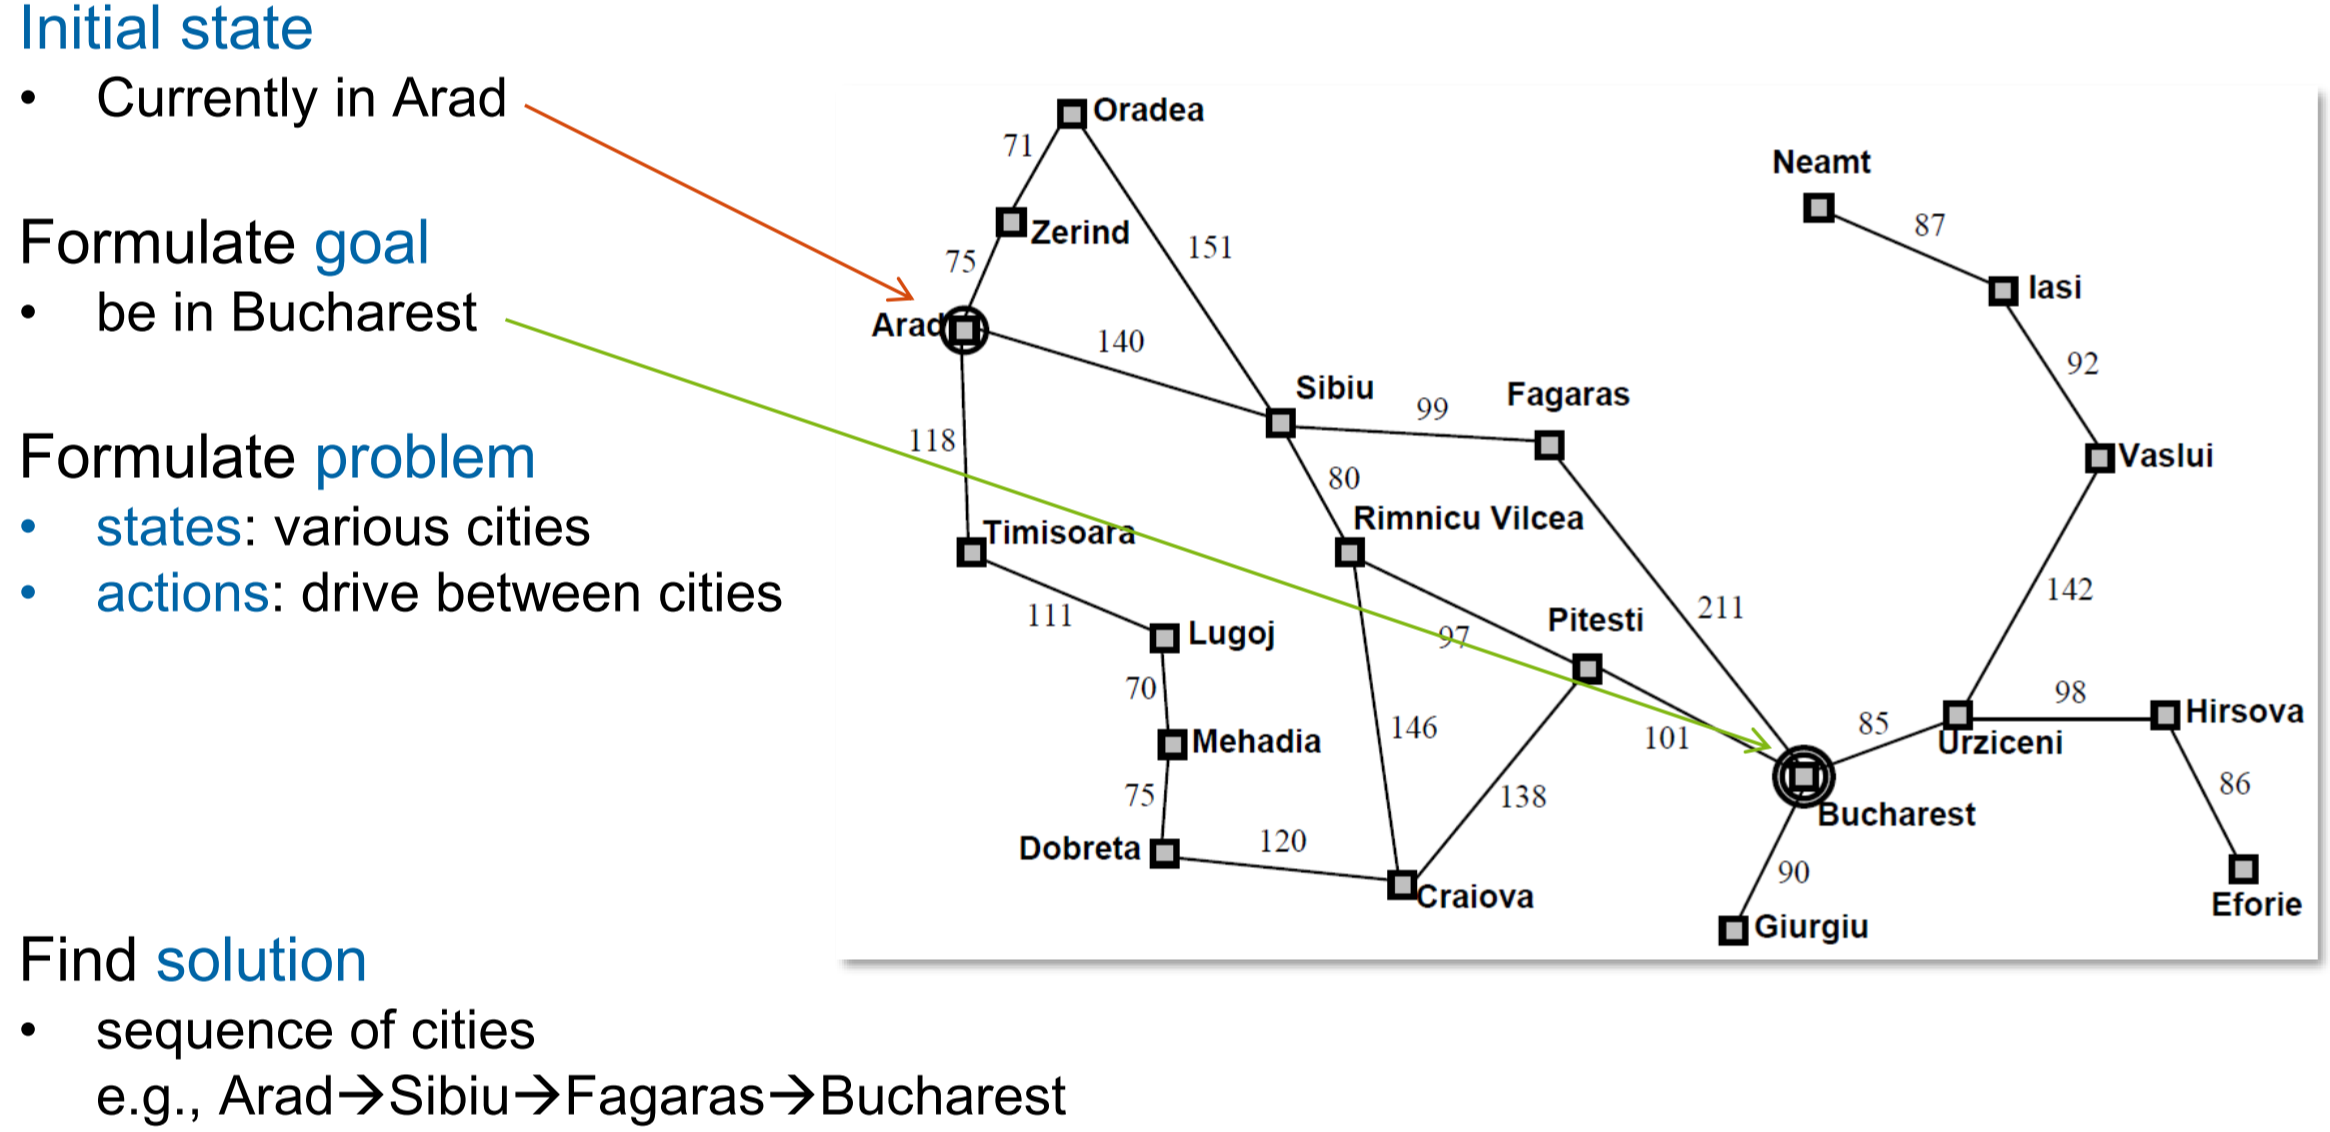
\includegraphics[width=300px]{img/SearchingAsProblemSolvingGPS.png}
	\captionof{figure}{Real-World Beispiel für eine Baumsuche}
	\label{fig:Real-World Beispiel für eine Baumsuche}
\end{Figure}

\textbf{geeigneten Suchagenten strukturieren}\\
Dabei soll der Agent so aufgebaut werden, dass sich "die Welt" darin wieder findet.\\
\textit{Offline problem solving} bedeutet, dass man das Problem simulieren kann. Dagegen ist die Online Problemlösung bspw. das effektive Abfahren der Strecke.
\begin{Figure}
centering
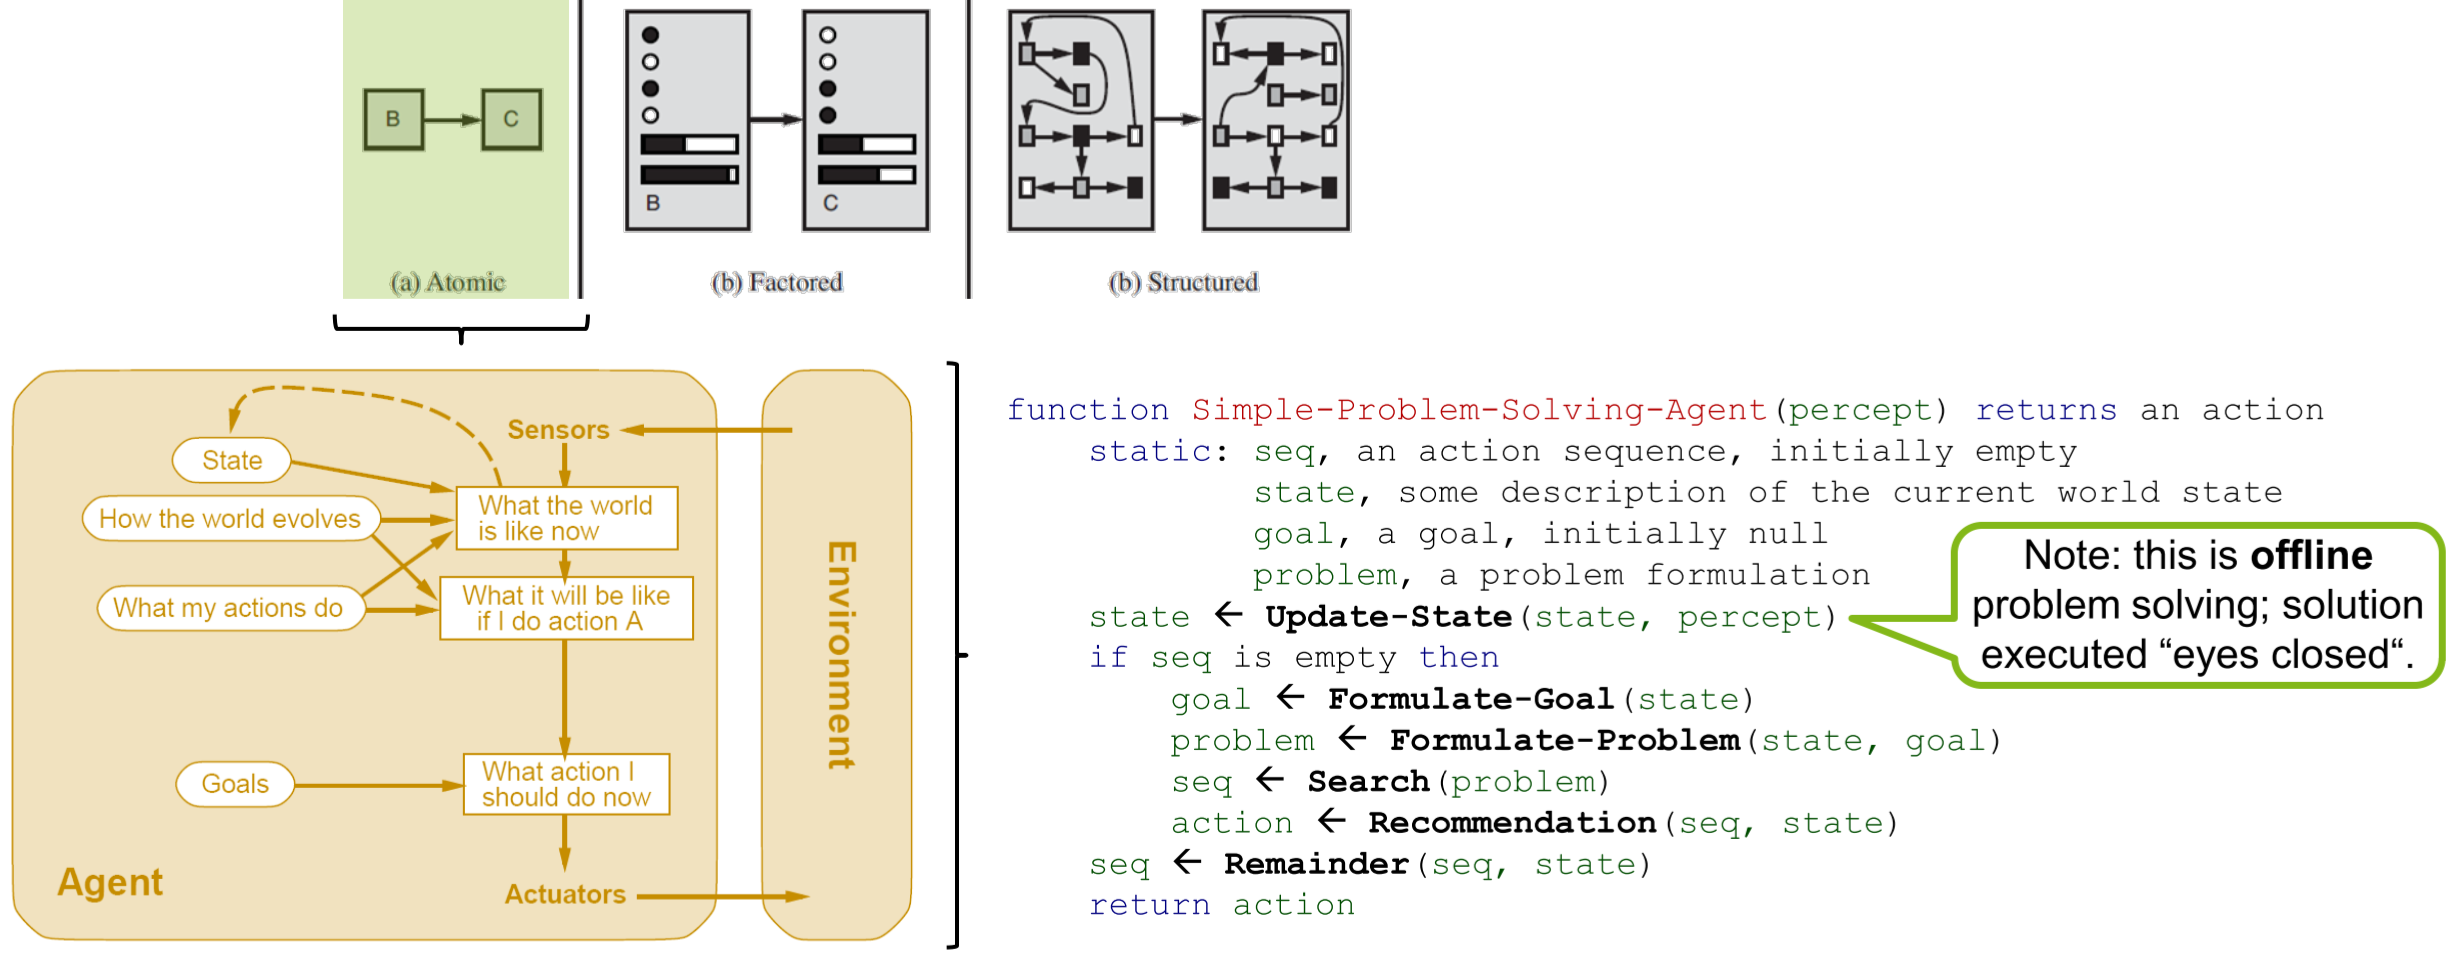
\includegraphics[width=400px]{img/suitableAgentStructure.png}
	\captionof{figure}{Möglicher Aufbau eines modellbasierten Agenten}
	\label{fig:Möglicher Aufbau eines modellbasierten Agenten}
\end{Figure}

\subsubsection{Verschiedene Ansätze der Suche}
\begin{itemize}
\item{\textbf{uninformed (blind) search} Man ist blind, man kann nicht abschätzen, welcher Ansatz der besser ist. Dementsprechend muss man alle Ansätze durchgehen und am Schluss entscheiden, was der bessere isch. Vor allem geeignet bei: fully observable, deterministisch und diskret}
\item{\textbf{heuristic} Kennt den nächsten Status. Vor allem geeignet bei: identisch wie uninformed, jedoch grösser}
\item{\textbf{Online Search} für Umgebungen, welche dynamisch sind}
\item{\textbf{local search} fokusiert sich auf das Finden des Ziels und nicht auf den optimalen Pfad}
\item{\textbf{adversial search} ist die Suche wenn man einen Gegner hat, bspw. Schach} 
\end{itemize}

\subsection{Uninformed / blinde Suche}
Ist eine Baumsuche, welche alle Knoten des Baums gesucht wird. Evaluationkriterien für die Strategie folgende:
\begin{itemize}
\item{complet findet der Algorithmus immer eien Lösung}
\item{optimal, findet der Algorithmus jeweils die Lösung mit den geringsten Kosten}
\item{Zeit-Komplexität, Anzahl der Knoten (generated/expaneded}
\item{Speicherplatz-Komplexität, maximale Anzahl an Knoten im Speicher}
\end{itemize}

\textit{Zeit und Speicher Komplexität sind gemessen in}\\
\begin{itemize}
\item{\textit{b:} maximum branching factor of the search tree}
\item{\textit{d:} Tiefe der Kostengünstigste Lösung}
\item{\textit{m:} maximum depth of the state space (may be infinity}
\end{itemize}
\begin{Figure}
centering
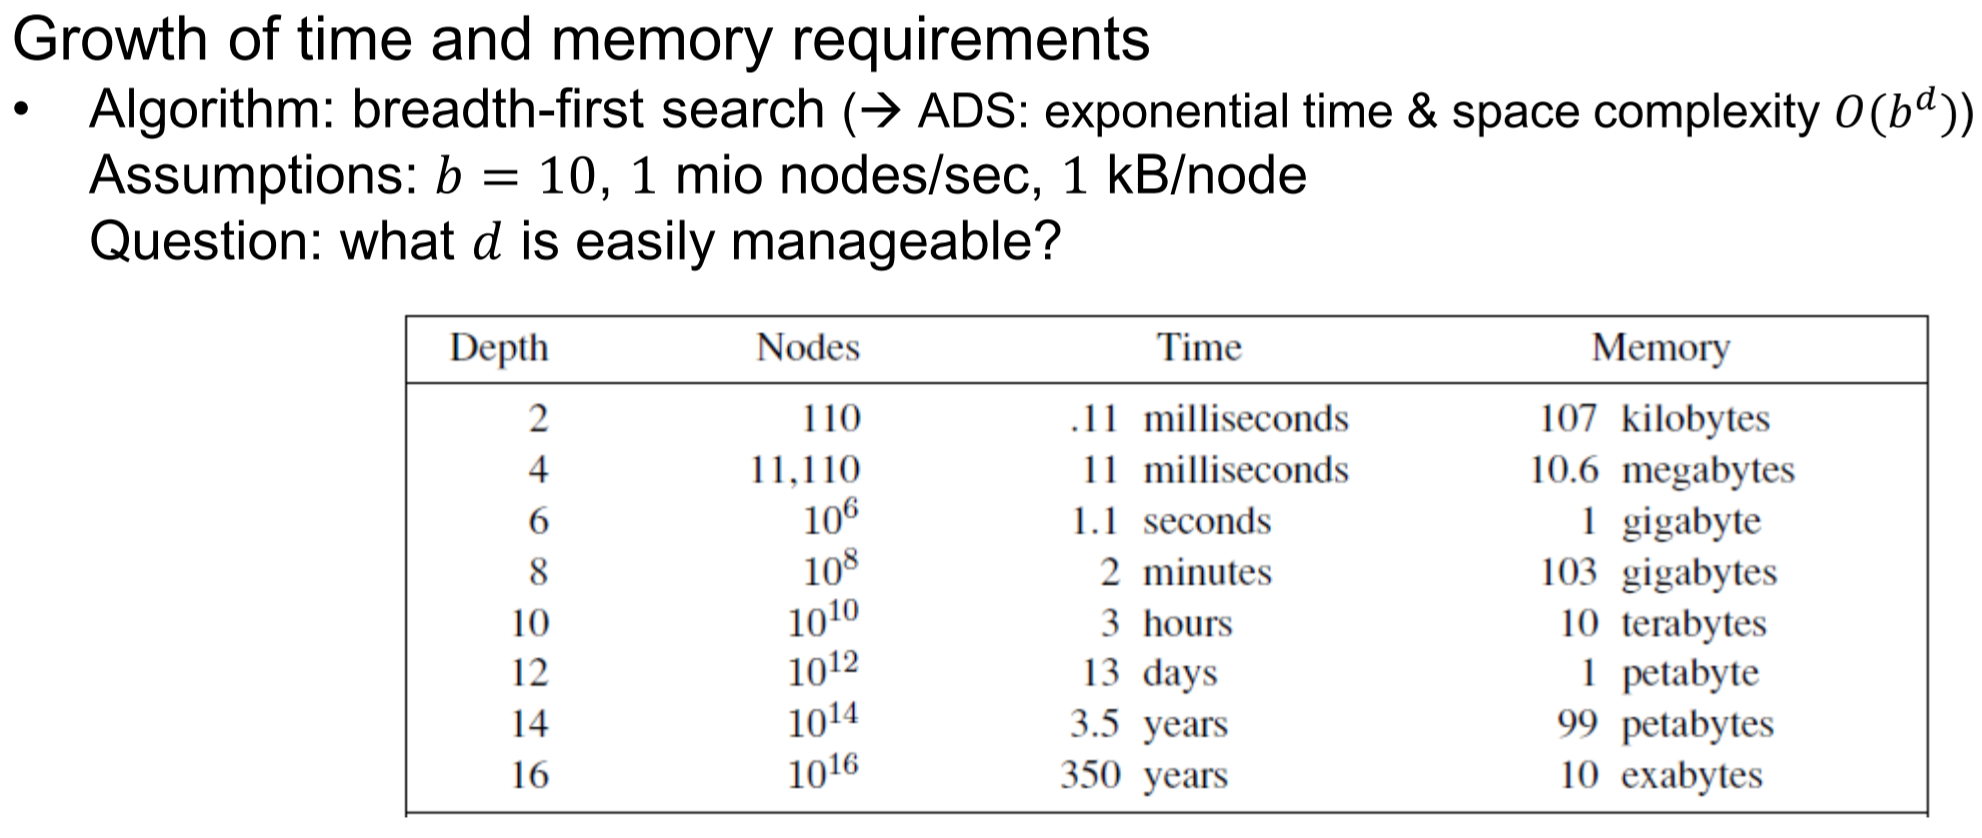
\includegraphics[width=400px]{img/uninformedSearch.png}
	\captionof{figure}{Live Beispiel einer blinden Suche}
	\label{fig:Live Beispiel einer blinden Suche}
\end{Figure}

\textit{Strategien für die blinde Suche}\\
\begin{itemize}
\item{\textit{Tiefensuche} tbd}
\item{\textit{Breitensuche} tbd}
\item{\textit{Uniform-Cost} tbd}
\item{\textit{limitierte Tiefensuche} tbd}
\item{\textit{Iterative Deepening} Mix aus Tiefen- und Breitesuche, da es auch die Vollständigkeit und Optimalität widerherstellt}
\end{itemize}
\begin{Figure}
centering
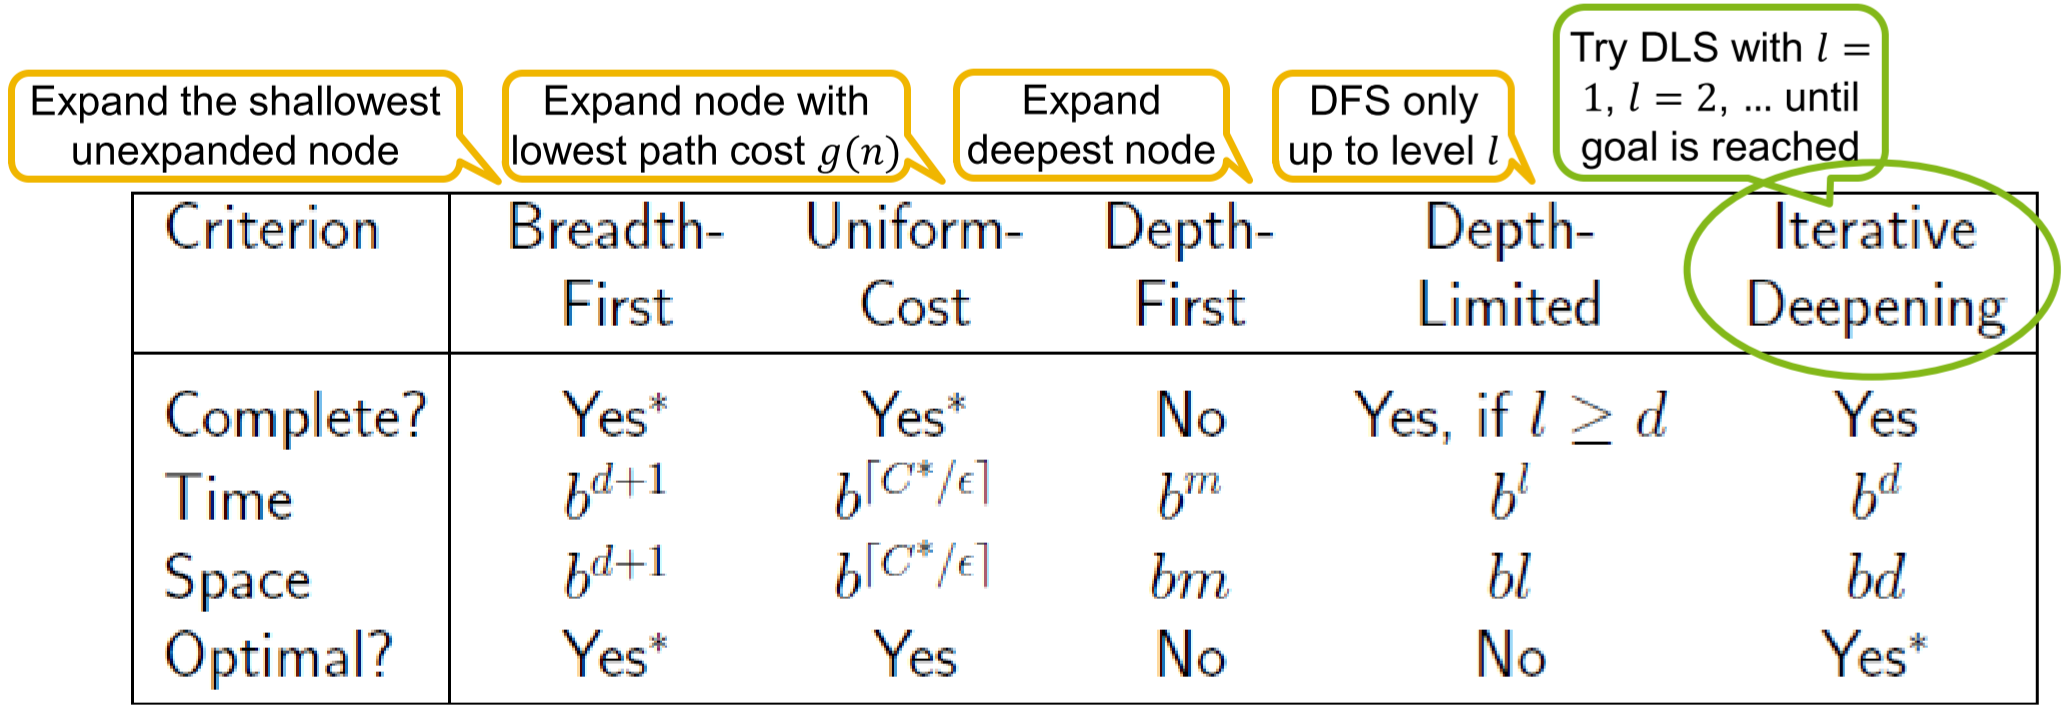
\includegraphics[width=400px]{img/uninformedSearchStrategies.png}
	\captionof{figure}{unterschiedliche Strategien für die blinde Suche}
	\label{fig:unterschiedliche Strategien für die blinde Suche}
\end{Figure}

\subsection{heuristische Suche}
Man hat eine Möglichkeit einen Zustand zu bewerten und abzuschätzen, ob man mit diesem Zustand näher am Ziel ist als ein anderer Zustand oder einen vorherigen Zustand.\\
Ein möglicher Ansatz ist die \textbf{best-first-Suche}:\\
\begin{itemize}
\item Wähle den nächsten Node aus, basierend auf einer definierten Funktion $f(node)$
\item Typischerweise ist f, als Heuristik $h(node)$ implementiert
\item $h(node)$ facillitates pruning of the search tree
\end{itemize}

\subsubsection{typische Implementationen}
\textbf{Greedy Search}
\begin{itemize}
\item{immer den günstigen Weg nehmen zum nächsten Node}
\item{tbd}
\end{itemize}

\textbf{A\*}
\begin{itemize}
\item{A\* $\rightarrow$ man nimmt den günstigen Weg, berücksichtigt jedoch noch den bereits zurückgelegten Wert}
\item h(n) needs to be admissible: \textbf{tbd}
\item A\* ist optimal und komplett
\item A\* hat die Zeit-Kompexität $O(2'{error of h) * d}$
\end{itemize}

\textbf{SMA\* - simplified memory-bounded A\*}
\begin{itemize}
\item{A\* braucht meistens zu viel Speicherplatz, da kommt dann der SMA ins Spiel}
\item{tbd}
\end{itemize}























 \end{document}